\chapter{Expresiones regulares} \label{chap:regex}

En este anexo se exponen los distintos grupos de captura que definen la expresión regular para el parseo de chats exportados por WhatsApp, tanto desde Android como iOS.

\begin{figure}[h]
	\centering
	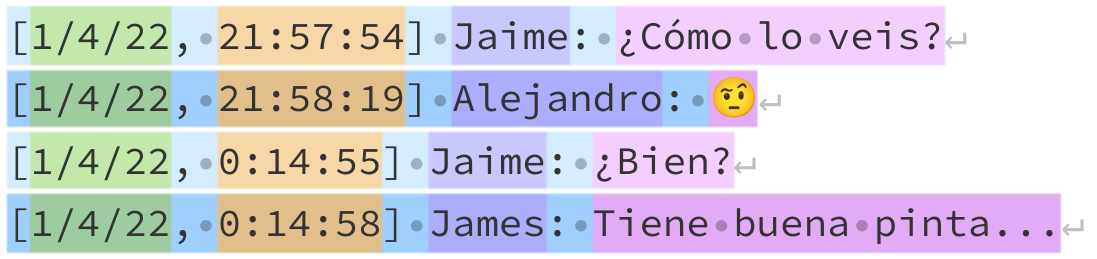
\includegraphics[width=0.6\textwidth]{img/regex_ios.png}
	\caption{Grupos de captura iOS en color}
	\label{fig:chap:regex_ios}
\end{figure}

\begin{figure}[h]
	\centering
	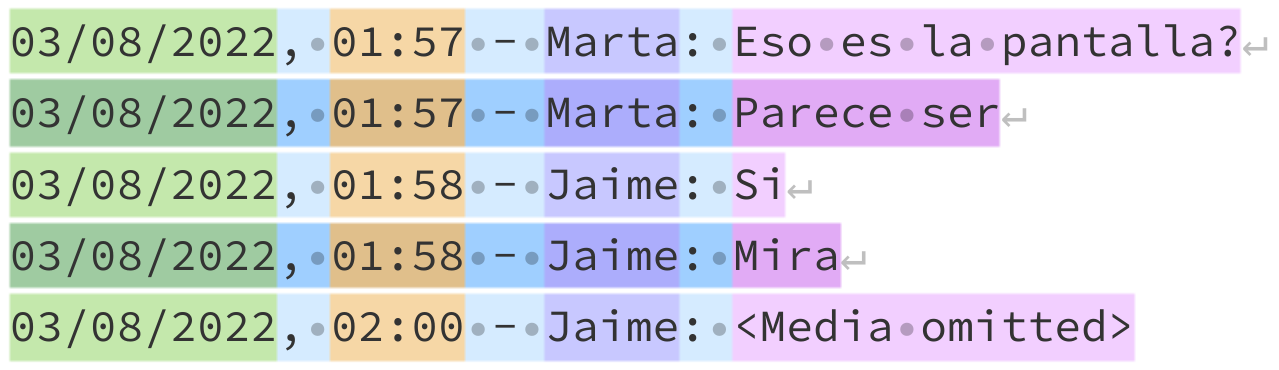
\includegraphics[width=0.6\textwidth]{img/regex_android.png}
	\caption{Grupos de captura Android en color}
	\label{fig:chap:regex_android}
\end{figure}

\section{Grupos de captura}

Como se decribe en el \autoref{chap:architecture}, poder separar cada mensaje se ha llegado a la siguiente expresión regular, cuyos grupos se explicaran a continuación:

\begin{lstlisting}
	/\[*(\d{1,2}\/\d{1,2}\/\d{2,4}),\s(\d{1,2}:\d{2}:*\d*)\]*\s(?:-\s)*(.*?):{1}\s(.*?)(?=\s\[*\d{1,2}\/\d{1,2}\/\d{2,4}|$)/gum
\end{lstlisting}

Se denotan los distintos grupos de captura por las agrupaciones realizadas con los paréntesis. Se exponen:

\paragraph{Grupo de captura 1: fecha}\mbox{}\\

\begin{lstlisting}
	(\d{1,2}\/\d{1,2}\/\d{2,4})
\end{lstlisting}

Se encarga de la fecha en formato \textit{dd/mm/YYYY} para Android y \textit{d/m/YY} para iOS; denotado con ``$\backslash d\{X,Y\}$'' que indica que se buscan entre $X$ e $Y$ dígitos de $0$ a $9$ seguidos, separados por un ``$/$''. En las expresiones regulares hay que escapar los ``$/$'' o \textit{slash} con un ``$\backslash$'' o \textit{backslash}.

Durante numerosas pruebas, se ha observado que no hay consistencia entre los ajustes del parámetro \textit{locale} de \textit{en\_US} y \textit{es\_ES}, siendo \textit{mm/dd/YYY} y \textit{dd/mm/YYYY} respectivamente. Para ello, ChatStats accederá al \textit{locale} para actuar en consecuencia más adelante. No se ha probado para otras configuraciones.

Puede observarse en verde en la \autoref{fig:chap:regex_android} y \autoref{fig:chap:regex_ios}.

\paragraph{Grupo de captura 2: hora}\mbox{}\\

\begin{lstlisting}
	(\d{1,2}:\d{2}:*\d*)
\end{lstlisting}

Se encarga de la la hora en formato \textit{hh:MM} para Android y \textit{h:M:ss} para iOS, donde en caso de comenzar por 0, este no se muestra. Es por ello que se esperan entre 1 y 2 dígitos para la hora y los minutos, así como el parámetro de los segundos es opcional. Este último parámetro, si existe, siempre está conformado por dos números.

Puede observarse en naranja en la \autoref{fig:chap:regex_android} y \autoref{fig:chap:regex_ios}.

\paragraph{Grupo de captura 3: contacto}\mbox{}\\

\begin{lstlisting}
	(.*?)
\end{lstlisting}

Se encarga del nombre del contacto. Busca la repetición de caracteres ilimitados a excepción del carácter ``\textit{:}'', ya que éste es un separador.

Puede observarse en azul oscuro en la \autoref{fig:chap:regex_android} y \autoref{fig:chap:regex_ios}.

\paragraph{Grupo de captura 4: mensaje}\mbox{}\\

\begin{lstlisting}
	(.*?)
\end{lstlisting}

Se encarga del cuerpo del mensaje. Busca la repetición de caracteres ilimitados, incluyendo caracteres unicode para tener los emoticonos en cuenta. Esta búsqueda de caracteres se realiza de manera perezosa, expandiendo las coincidencias en caso posible, siempre que no coincida con el siguiente grupo de captura (\textit{lookahead}).

Puede observarse en rosa en la \autoref{fig:chap:regex_android} y \autoref{fig:chap:regex_ios}.

\paragraph{Look ahead o mirada hacia delante}\mbox{}\\

\begin{lstlisting}
	(?=\s\[*\d{1,2}\/\d{1,2}\/\d{2,4}|$)
\end{lstlisting}

Si únicamente contáramos con el grupo de captura 4, solo se reconocería el primer mensaje, puesto que se reconocería el resto del texto como cuerpo del primer mensaje. Para solucionarlo, en el grupo de captura 4 se intentan reconocer el menor número posible de coincidencias, hasta el siguiente patrón reconocido. Este patrón es una mirada hacia delante conformada por la misma expresión regular que en el grupo de captura 1.

\paragraph{Opciones}\mbox{}\\

\begin{lstlisting}
	\gum
\end{lstlisting}
 
Finalmente se aplican tres opciones a la expresión regular, que son:

\begin{itemize}
	\item \textbf{g:} Nos permite no terminar la búsqueda de patrones tras la primera coincidencia.
	\item \textbf{u:} Nos permite la búsqueda de caracteres unicode, así como emojis (que pertenecen a la especificación unicode).
	\item \textbf{m:} Nos permite realizar la búsqueda en numerosas líneas, pudiendo encontrar coincidencias con mensajes de varias líneas.
\end{itemize}